% Name: Slope field
% Description: The slope field of the differential equation dy/dx = x − y, with three solution curves y = x − 1 + Ce⁻ˣ following the slopes.
% Tags: slope field, direction field, differential equation, solution curves

\usetikzlibrary{arrows.meta}

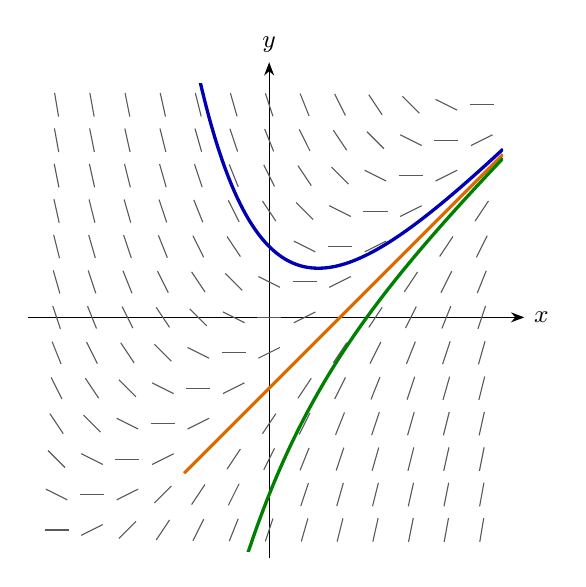
\begin{tikzpicture}[>={Stealth}, scale=0.9, every node/.style={font=\small}]
  \draw[->] (-3.4,0) -- (3.6,0) node[right] {$x$};
  \draw[->] (0,-3.4) -- (0,3.6) node[above] {$y$};
  % At each grid point, a short segment with the slope x - y
  \foreach \x in {-3,-2.5,...,3} \foreach \y in {-3,-2.5,...,3} {
    \pgfmathsetmacro\a{atan(\x - \y)}
    \draw[gray!70!black, thin] ({\x - 0.17*cos(\a)}, {\y - 0.17*sin(\a)}) -- ({\x + 0.17*cos(\a)}, {\y + 0.17*sin(\a)});
  }
  \clip (-3.3,-3.3) rectangle (3.3,3.3);
  \foreach \C/\c in {2/blue!70!black, 0/orange!85!black, -1.5/green!50!black}
    \draw[very thick, \c, domain=-1.2:3.3, samples=60, smooth] plot (\x, {\x - 1 + \C*exp(-\x)});
\end{tikzpicture}
